
\section{Design of the proposed solution}\label{ch:design}

This section describes the design of our proposal to integrate IoT constrained devices as part of the privacy preserving ecosystem P2ABCE. The ultimate goal is to enable constrained IoT devices to play the Idemix User and Verifier roles, interacting autonomously in order to authenticate and demonstrate their credential attributes to any Verifier in a privacy-preserving fashion, as well as verifying other devices in a M2M environment, addressing the power and memory constrains many IoT devices face. 

Applying Anonymous Credentials Systems in IoT constrained devices enables a new vast range of opportunities and scenarios that have not being addressed so far. For example, controlled access doors where the access control lists (ACLs) are stored in the constrained terminals. A user may present in a M2M fashion a zero-knowledge proof of her being authorized by the list, the terminal then acts as a ACS Verifier to open or not the door. It avoids querying to an external trust party to verify the attributes, gives trust to the administrator that only authorized personnel can enter, and gives trust to the Users that their activity is not stored in clear. 

As another example, a motorcycle could authenticate its owner by verifying a proof from her smart-watch. When parked, it could verify that another device is a policeman's authorized device, and in that case the vehicle would disclose its owner's relevant information, proof of passing technical inspections, etc. But when the vehicle is accessing a restricted residential area, it would provide a proof in a privacy-preserving fashion that its owner's address is within the area, without revealing the owner's identity or specific address where she lives. 


The project's requirements and objectives are structured below:

\begin{itemize}
	\item \textit{Security}: the solution should not compromise the security of the device's identities.
	\item \textit{Usability}: it should provide an API for developers to use the P2ABCE privacy capabilities in their applications.
	\item \textit{Full P2ABCE support}: the IoT device should be capable of performing every action a traditional User or Verifier could perform.
	\item \textit{Transparent interactions}: any third party actor of the system should not be aware of the IoT condition of the device, therefore, there should be no changes to the P2ABCE protocol.
	\item \textit{Constrained devices}: the solution should aim to be portable and applicable to as many IoT devices as possible, including those with less computing capabilities.
\end{itemize}

\hfil

To address these objectives, considering the evolution of Identity Mixer to use smart cards, our solution will consist on a mandatory implementation of the smart card logic inside the IoT device, which will conceal all the operations regarding secret keys, and to manage the P2ABCE language, the solution shall offer an API which, at the time being, will perform \textit{computation offloading} to a device capable of running the framework.

Even in the case all P2ABCE were to be implemented inside an IoT device, it should implement the support for software smart cards, to keep the secret inside the IoT device. Therefore, the first step is to implement the smart card logic inside the IoT device, and later, if the device resources admit it, other components of the P2ABCE framework.

Computation offloading is not a new technique for IoT environments. For example, to reduce the overhead of IPv6, 6LoWPAN compresses packets and uses smaller address sizes. In order to communicate a 6LoWPAN with other networks, the IoT devices delegate on a proxy that can manage the 6LoWPAN and IPv6 stacks. In the scope of consumer devices, smart watches can install applications which delegate on the user's phone to accomplish performance demanding task. 
Therefore, the IoT device now has a \textbf{duality} in its functions, because it is the User that starts any interaction with other actors, and it is also the smart card that a P2ABCE server must ask for cryptographic operations. It can also be seen as a \textbf{double delegation}. The IoT device delegates on the external P2ABCE server to manage the protocol, and that P2ABCE server delegates on the IoT device, acting now as the smart card.

Regarding the communication between different P2ABCE actors, it depends on each IoT scenario, independently of our solution, as third party actors have no need to adapt the P2ABCE protocol.



% TODO mencionar más adelante qué se ha conseguido de cada
% Security : el canal seguro y autenticado entre servidor y IoT, así como mantener la IoT smart card segura
% Usability : el toolkit permite al fabricante usarlo como una API y usar el despliegue que prefiera, actuando como recipient al inicio
% Full support & transparent : el parser se ejecuta en el servidor completo y se podría implementar en el dispositivo si la potencia lo permite
% Constrained : técnica de computation offloading

% TODO : escenarios de aplicación



To ensure that our solution does not risk the security of the device's secrets, the next section introduces the fundamentals on the operations performed by a User, therefore identifying the key operations to implement in the smart card.

\subsection{Fundamentals on Zero-Knowledge Proofs}

% Ejemplo de DL problem
% Firma CL
% Mostrar al final la estructura de la mayoría de ZKP : commitment(s), challenge, response(s)

To understand Zero-Knowledge Proofs, \textit{Fundamentals of Computer Security} \cite[Chapter 12]{book:856771} offers a good introduction to the topic. Here is shown how one can indeed proof knowledge of a value, without revealing it, using the classic ZKP of knowledge based on the discrete logarithm problem, also known as Schnorr's identification scheme. Based on this discrete logarithm ZKP, Idemix then derives multiple ZKPs of relations and properties of the values hidden in a credential.


Using the notation introduced by Camenisch and Stadler \cite{camenisch1997efficient}, the discrete logarithm ZKP can be written as 
\[ PK\{ (\alpha) : y = g^\alpha \}  \]
given a known group $G=\left\langle g \right\rangle $ of prime order $q$ and public value $y\in G$. The notation means: ``I know a secret value $\alpha$ such that $g^\alpha$ is $y$'', i.e. the discrete logarithm of $y$, $log_g y = \alpha$.


During the first step of the protocol, the prover chooses randomly a value $r$, computes the \textit{commitment} $t := g^{r}$ and sends $t$ to the verifier. 
Then, the verifier chooses another random exponent, the \textit{challenge} $c$, and sends it to the prover. 
Next, the prover computes the \textit{response} $s:=r-c\alpha\, mod\, q$ and sends it to the verifier.
Finally, the verifier checks whether or not $ t \overset{?}{=} g^{s} y^c $ holds. The verifier never receives the secret value $\alpha$, and the verifier will not be able to compute it given $t$ and $s$.

The protocol holds because $ g^{s} y^c  =  g^{r - c\alpha} g^{\alpha c} = g^{r} = t $.

\begin{figure}[bth]
	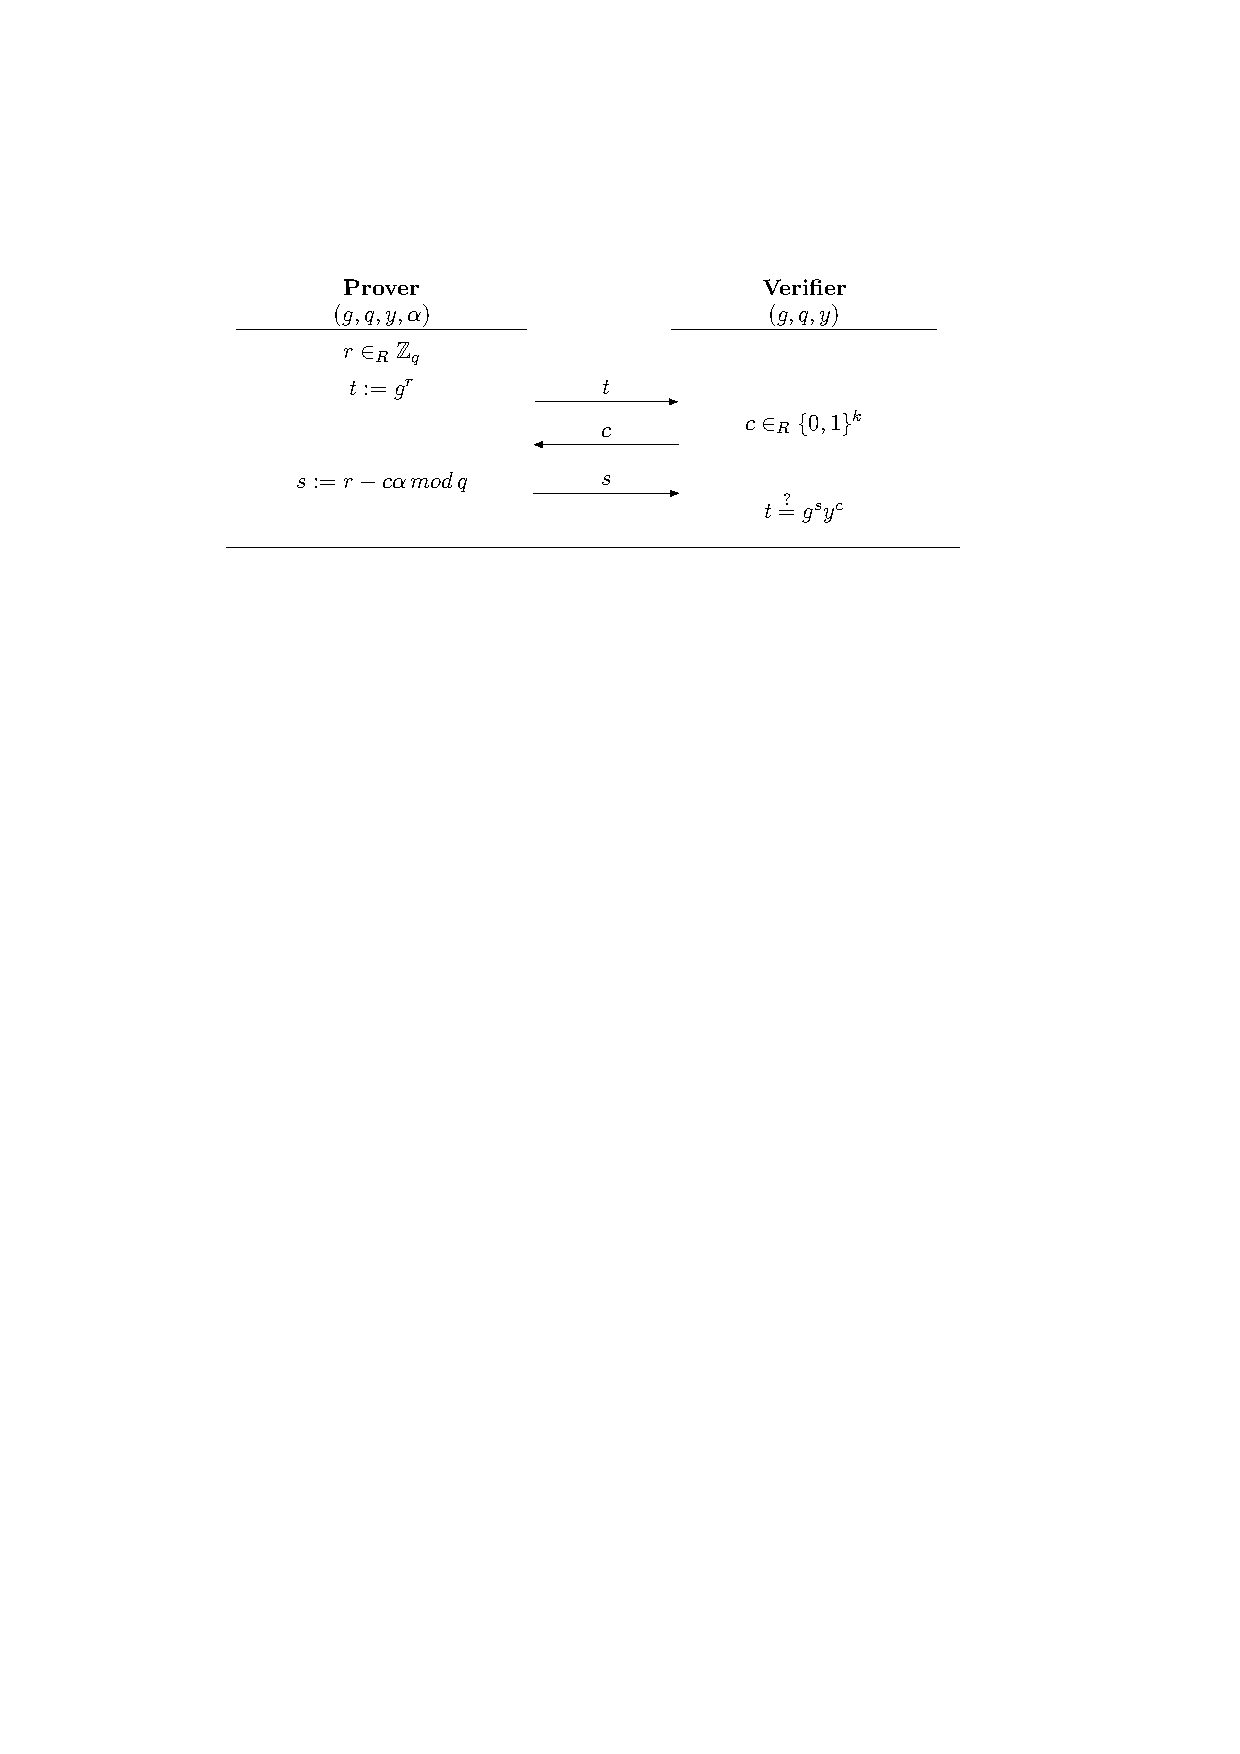
\includegraphics[width=\linewidth]{gfx/schnorr}
	\caption{Schnorr's protocol $PK\{ (\alpha) : y = g^\alpha \}$. The prover knows $(g,q,y,\alpha)$ such that $g^\alpha=y$. The verifier knows $(g,q,y)$.}
	\label{fig:schnorr}
\end{figure}

The Fiat-Shamir heuristic lets us replace the verifier challenge with a hash function $\mathcal{H}$, computing the challenge as $c:=\mathcal{H}(g\mid y\mid t\mid n)$. The value $n$ is a random nonce generated by the verifier at the beginning of the non-interactive ZKP. The nonce makes the verifier trust that the current ZKP is fresh and not a forgery from a previous ZKP.

In Idemix, every ZKP follows the scheme shown above. First, we have the \textit{commitment} \texttt{t}, next the \textit{challenge} \texttt{c} (computed with $\mathcal{H}$), and finally, the \textit{response} \texttt{s}. A prover can achieve parallel ZKPs if she first computes the multiple \texttt{t}-values of each individual proof, next, she computes the same challenge \texttt{c} for all the proofs by combining all the information in one hash call, and then she computes all the \texttt{s}-values in parallel.

\begin{figure}[bth]
	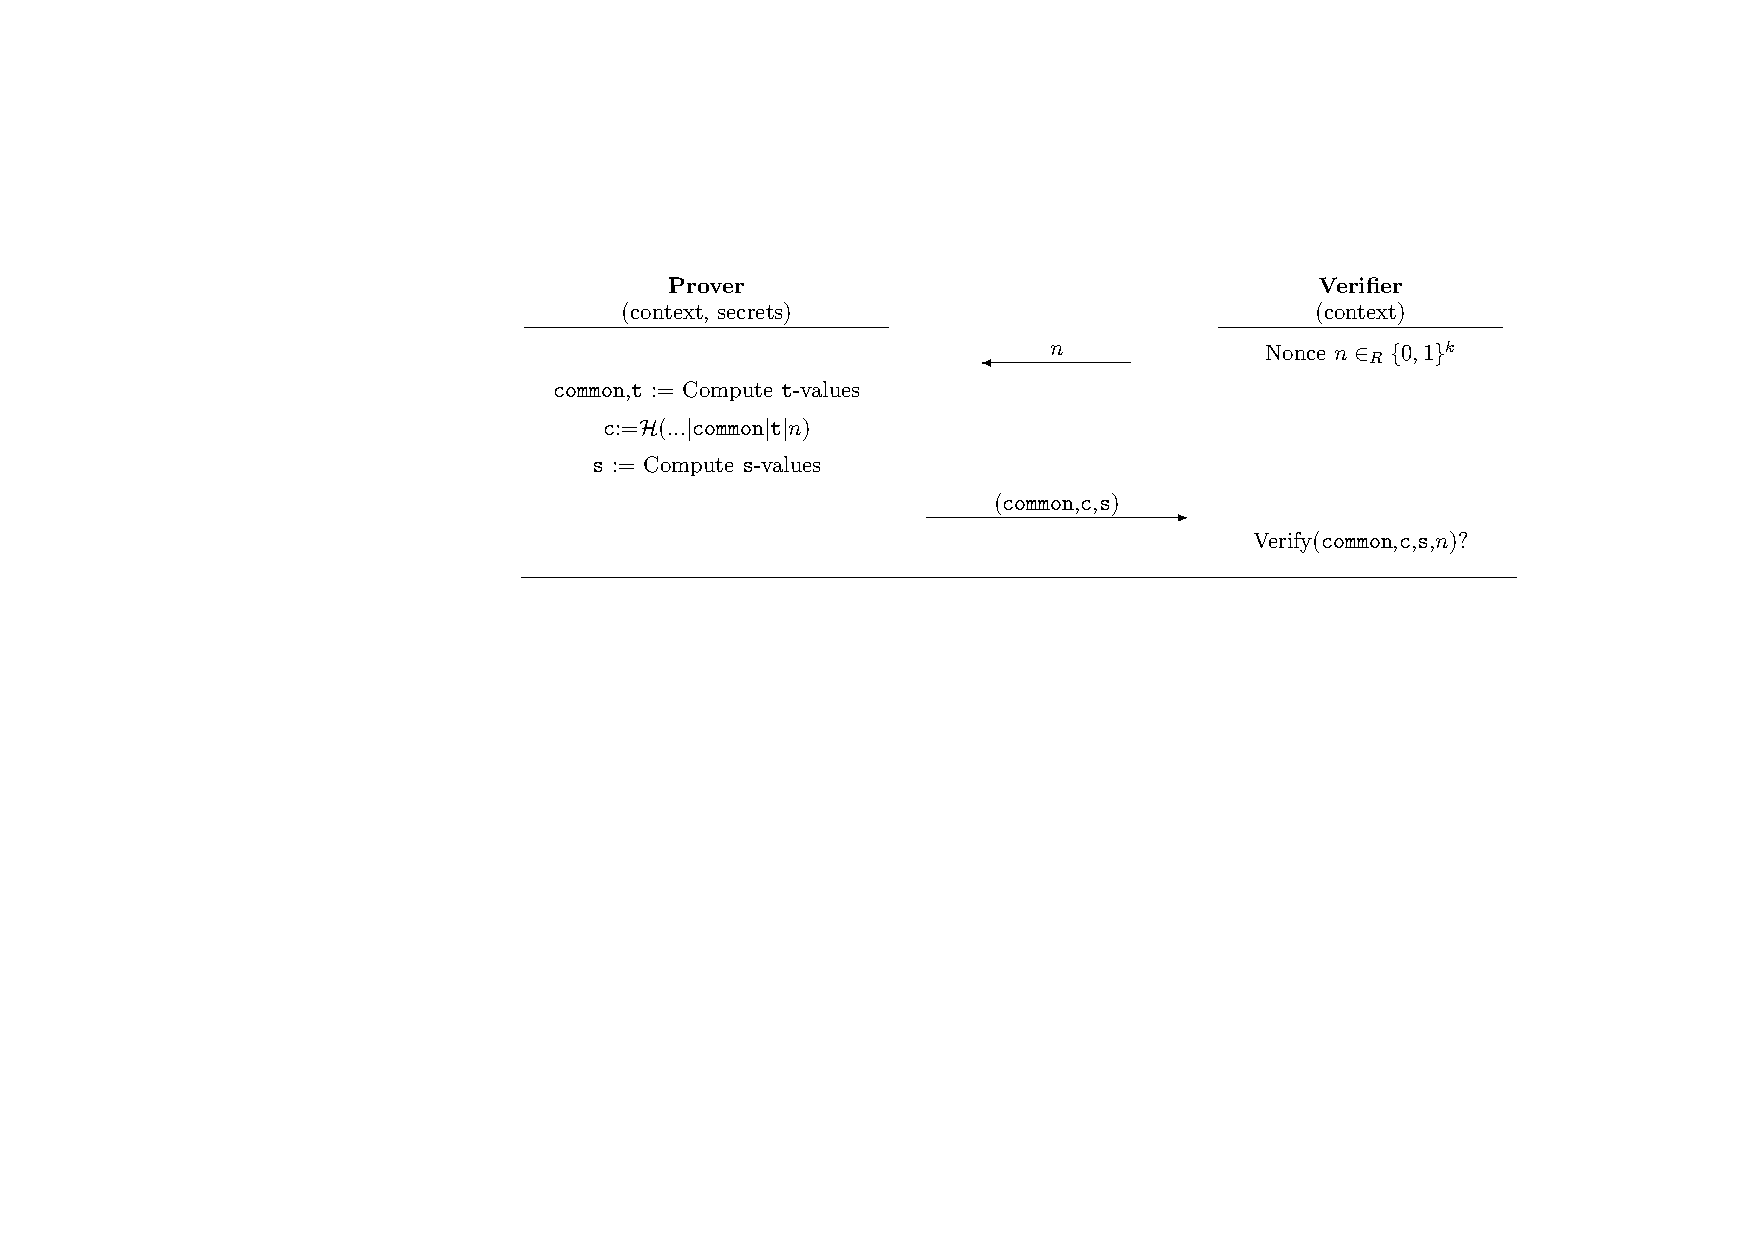
\includegraphics[width=\linewidth]{gfx/niZKPnonce}
	\caption{Identity Mixer's Non-Interactive ZKP with Nonce.}
	\label{fig:niZKPnonce}
\end{figure}

Fig. \ref{fig:niZKPnonce} shows the Idemix Proving scheme, where prover and verifier share a context information, the verifier generates the nonce, and the prover, non-interactively, computes the proof. The \texttt{common} values are equivalent to Schnorr's $t$, which was shared between prover and verifier. The verifier can recover some \texttt{\^t}-values from \texttt{common}, \texttt{c} and the \texttt{s}-values. This is equivalent to recovering Schnorr's $t$ from $g^{s} y^c$. The verifier then checks whether or not \texttt{c} equals $\mathcal{H}$(...$\mid$\texttt{common}$\mid$\texttt{\^t}$\mid$$n$) to verify if the \texttt{\^t}-values are actually the \texttt{t}-values, making the proof valid.


Therefore, to describe any Idemix proof being performed by the User, one can focus on the key steps, compute the \texttt{t}-values, the challenge \texttt{c} and the \texttt{s}-values, and ignore the mathematical operations performed for each specific ZKP.



\subsection{System architecture}

The system will be compounded by the IoT device, the P2ABCE delegation server and the third party P2ABCE actors:

\begin{figure*}[htb!]
	\centering
	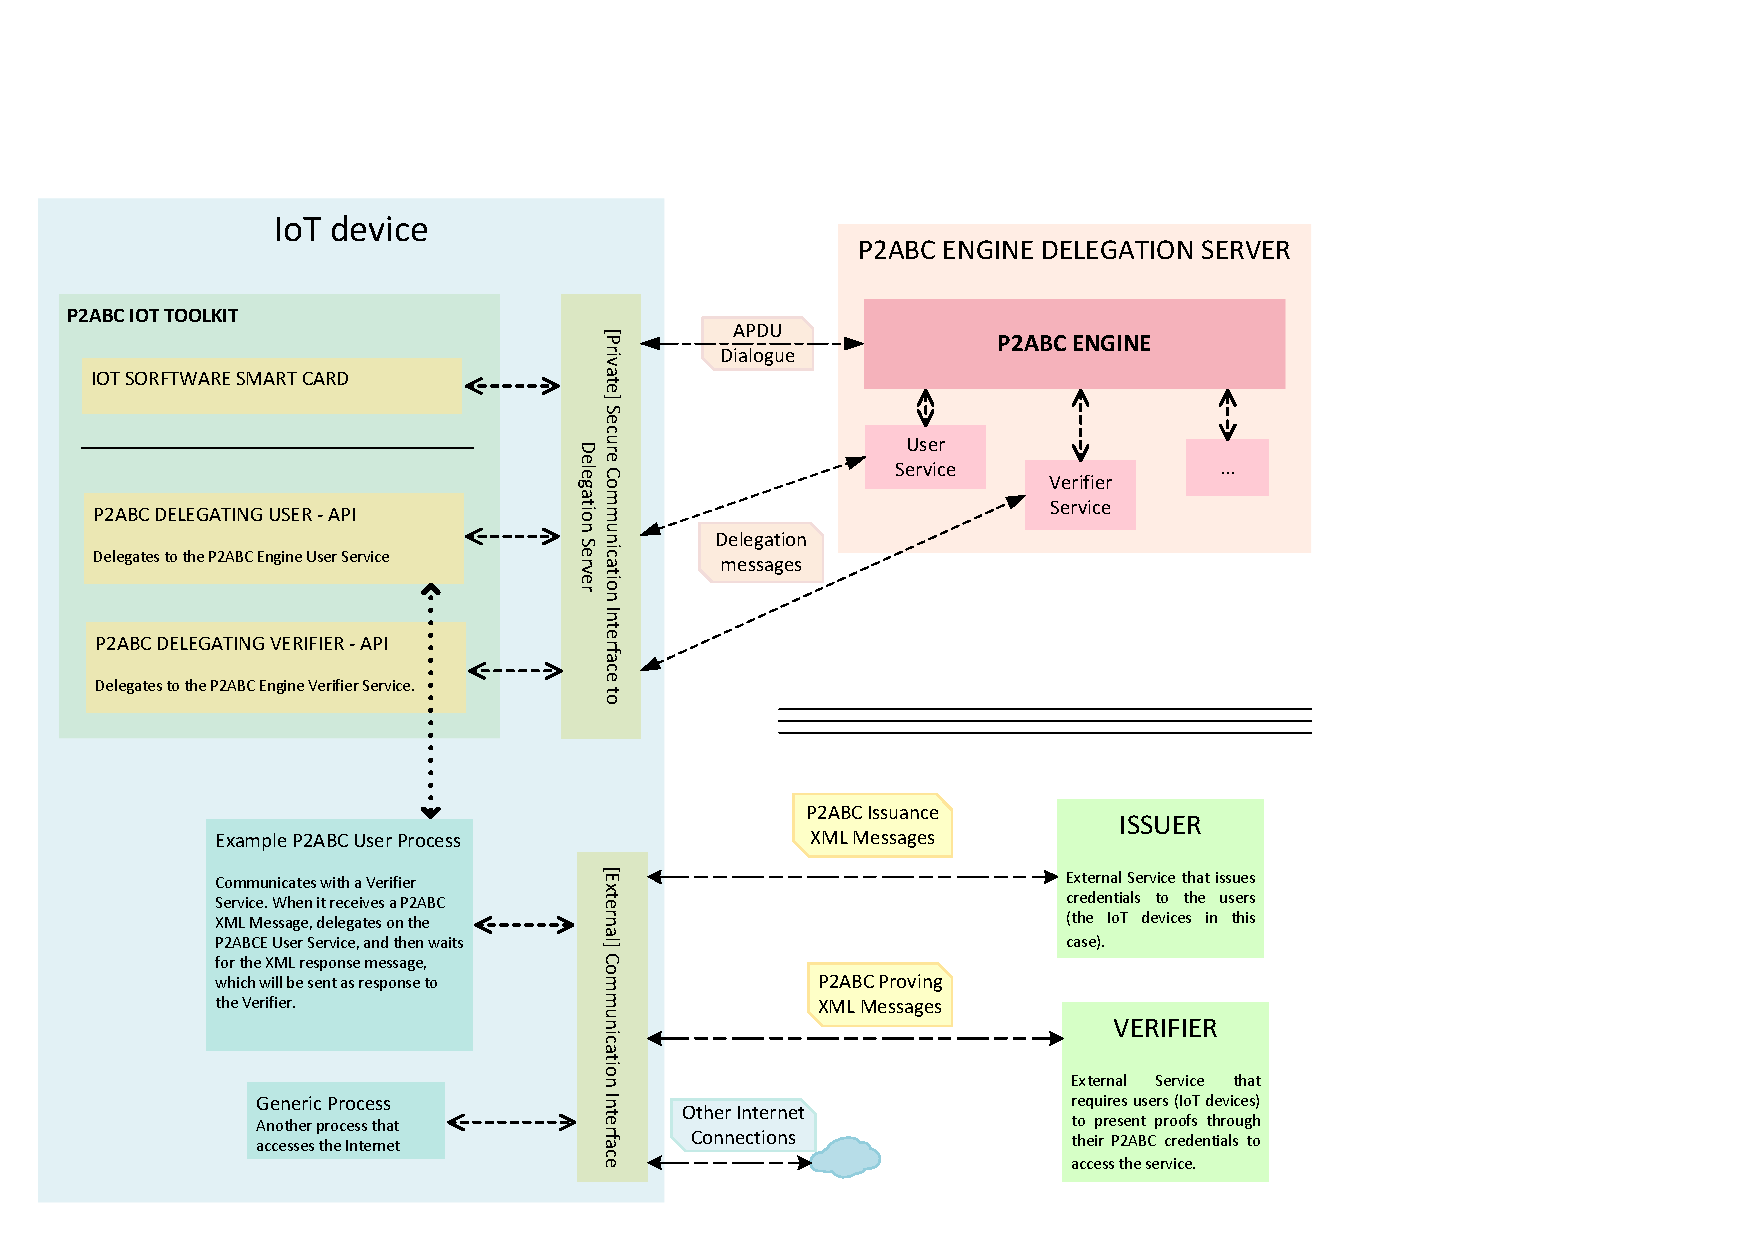
\includegraphics[width=0.7\textwidth]{gfx/P2ABCE-IoT-color}
	\caption{Proposed high level Architecture for integrating IoT devices in P2ABCE.}
	\label{fig:P2ABCE-IoT}
\end{figure*}



\begin{flushleft}
	\textbf{IoT device}:
\end{flushleft}

Figure \ref{fig:P2ABCE-IoT} shows our proposed architecture, in which the IoT device is represented with two communication interfaces. One allows external communications to other machines, including other P2ABCE actors. Through this interface, the P2ABCE XML messages are exchanged as in any traditional P2ABCE scenario. This lets an IoT device to interact with other actors without adaptations of the protocol. The other interface allows a secure communication channel with the delegation server. Both the delegation messages and the APDU Dialogue are transmitted over this interface, making it a point of attack that must be thoroughly secured.

The scheme also shows the \textit{P2ABCE IoT Toolkit}. This piece of software includes the \textit{IoT Smart Card}, and the P2ABCE API.

The \textit{IoT Smart Card} is the implementation of a software smart card, which listens for APDU Commands from the secure interface and stores the credentials and private keys within the device's memory. 
These secret keys should be kept securely protected inside the IoT smart card. There exist different software solutions, as well as hardware, like Atmel's chips, which offer secure memory and cryptographic operations, with serial interfaces for the IoT devices. Those chips also allow to speed up the SHA256 and AES128 calculations when compared with the performance obtained using software implementations.

The P2ABCE API is an interface for other processes that wish to use the private-preserving environment of P2ABCE. It provides access to every operation available, hiding the delegation process to the server. In the future, for example, the Verification Service could be implemented to run entirely in the IoT device, then the toolkit would conceal the transition from delegation to native execution.

\hfil

\begin{flushleft}
	\textbf{P2ABCE actors}:
\end{flushleft}

The possible roles in a P2ABC system are the Issuer, the User, the Verifier, the Revocation Authority and the Inspector, where these last two actors are optional. All of them use the P2ABCE language to communicate to each other. Any third party actor that communicates with the IoT device will be unaware of the fact that the device is a constrained device, because it will accept and generate the same XML as a traditional User.

Figure \ref{fig:actors} showcases the different actors and their interactions, where the User is in the center, which receives a credential from an Issuer, can generate privacy-preserving Tokens for Verifiers or revoke an stolen credential. The Inspector is the only entity capable of reading some ciphered attributes from a Token, if the User accepted to include that ciphered information in it. It serves the Law Enforcement authorities, warrant granted, to track any misuse of a credential.

\hfil

\begin{flushleft}
	\textbf{P2ABCE Delegation Server}:
\end{flushleft}

The machine in charge of receiving commands from authorized IoT devices to parse the XML files exchanged. It will also orchestrate through APDU Commands the cryptographic operations the IoT smart card must perform.


\begin{figure}[bth]
	\centering
	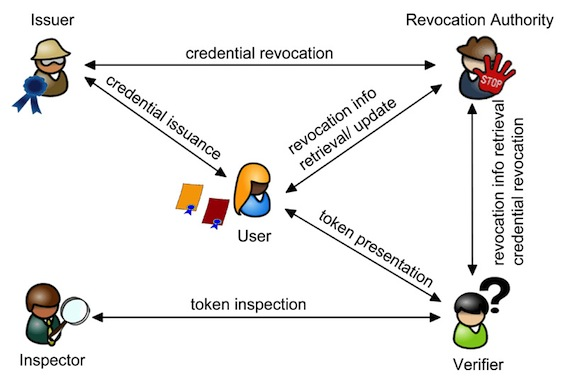
\includegraphics[width=0.8\linewidth]{gfx/actors.jpg}
	\caption{Entities in a P2ABC System. Source: P2ABCE project.}
	\label{fig:actors}
\end{figure}


\subsection{Delegation process}

This section describes the computation offloading carried out by the IoT device. The steps the device will perform in any kind of interaction are:

\begin{itemize}
	\item Communication with P2ABCE actor
	
	The IoT device, acting as a User, starts an interaction with another actor. If it is an Issuer, it will start the issuance process. If it is a Verifier, then it will provide a Presentation Policy for the device to proof in a privacy preserving way. Figure~\ref{fig:DelegationProving} shows an example of this last case.
	
	It may also happen that the device is contacted as a Verifier by another actor, e.g. in a M2M scenario where the IoT device requires authentication to access to its resources.
	
	\item Delegation to the P2ABCE Server
	
	Depending on what role the IoT device is acting as, it will use the corresponding API from the P2ABCE IoT Toolkit. The selected API will delegate to the Service deployed in the delegation server, e.g. User Service. The delegation message will include the XML data, and any parameter required to accomplish the task, as the information on how to communicate back with the IoT smart card.
	
	The server will then parse the XML messages and begin to orchestrate the response. In the case of the Verifier Service, it will answer immediately with an \textit{accept} or \textit{reject} of the Token. In case it is the User Service, it will need information from the IoT credentials and cryptographic operations.
	
	\item APDU Dialogue
	
	Through the secure channel between IoT device and server, the User Service will send APDU Commands to the  \textit{IoT smart card} to read the credential information or perform cryptographic operations involving private keys, necessarily stored inside the IoT device.
	
	During a proof, the Service will read the credential public information to fill the Presentation Token, and then will request the IoT smart card to calculate the \texttt{t}-values of the proof. The Service will read the \texttt{common} and \texttt{t}-values, use the nonce present in the Presentation Policy of the Verifier and compute the challenge \texttt{c}. Next, the Service will send \texttt{c} to the IoT smart card through another APDU Command to request the calculation of the \texttt{s}-values.
	
	After the APDU Dialogue, the Service has all the needed values to fill in the Token, and the IoT device performed all the operations involving private values on its own.
	
	
	\item Server response
	
	After the APDU Dialogue, if needed, the server may return a status code indicating success or failure, or a XML response if the third party actor requires an answer from the IoT device, as a Presentation Token, or the intermediate issuance messages.
	
\end{itemize}

\begin{figure}[bth]
	\centering
	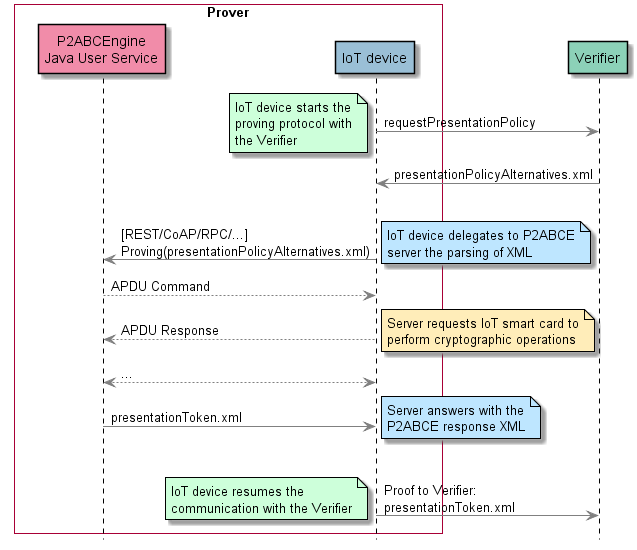
\includegraphics[width=\linewidth]{gfx/UML/provingDelegation}
	\caption{Messages exchanged during the proving delegation.}
	\label{fig:DelegationProving}
\end{figure}



The \textit{Server-IoT} channel must be secured. It must avoid impersonation of the P2ABCE delegation server or authorized devices. For this purpose many traditional solutions already exist. The delegation server could be in a local network, or physically attached to the IoT device, like the Arduino Y\'un\footnote{{https://www.arduino.cc/en/Main/ArduinoBoardYun}} combines an ATmega and an Atheros with Linux. The choice may depend on the particular deployment.

%Transmissions over the \textit{Server-IoT} channel must be secured in order to avoid attacks like impersonating the P2ABCE delegation server, an attacker sending APDU Commands to the IoT smart card, or delegating as a device to the server but giving the parameters of another device, making the delegation server send the APDU Commands to a victim IoT smart card.


%We could use a corporative PKI to issue certificates to the server and devices and configure policies for access control; design a challenge-response system combined with the smart card PIN, like a password and TOTP\footnote{Time-based One-time Password} in a 2FA\footnote{Two-factor authentication} login. We also could connect physically the delegation service through RS-232 serial to the IoT device, securing both physically as        we      would do with the IoT device on its own, isolating the delegation system from any network attack. % This last idea is an approximation to the Arduino Y\'un\footnote{\url{https://www.arduino.cc/en/Main/ArduinoBoardYun}}, a development board that integrates two microcontrollers, one a typical Arduino with very low resources, and another one running a fork of OpenWrt. The Arduino microcontroller can control the terminal of the more powerful one, using the serial pins as commented before.

%As      we        can see, there are many state of the art solutions for all this threads, therefore,           we       can assume a secure channel without mentioning a specific solution, providing freedom to choose the most fitting one in a real deployment.

%%%%%%%%%%%%%

%Regarding the definition of the P2ABCE API, it is a work in progress, and in the meantime,         we           will work with the REST API currently available in the P2ABCE project to perform the delegation. Regarding the \textit{IoT Smart Card}, the P2ABCE project defines the APDU instructions with the corresponding format of the APDU Commands and Responses. In the next section we will explain the PoC for IoT based on these P2ABCE specifications.



%%%%%%%%%%%%%